Based on the discussed practical applications and novel visualisation approaches, one can see that there is no such tool combining thematic maps with animations when changing visual appearance. The advantages and disadvantages of all aspects have been broached and discussed. This thesis will furthermore discuss and show a novel approach based on the concept of unit visualisations combined with classical thematic maps and animations when changing visual appearance. However, there are multiple possible solutions. This section will discuss some solutions with the requirement of building an interactive web application. The solutions should yield answers to the question of which tasks can be supported by particle aggregation in thematic maps and how can the aggregation be realized.

In order to realize a practical solution for the given question, it is assumed that a dataset including heterogeneous data and some kind of geospatial data is given.

According to the mantra of \citeauthor{Shneiderman1996}, the application should start by giving an overview of the dataset. With the main concept in mind, there are two possible solutions:
\begin{enumerate}

\ditem{Unit-based grid} \hfill \\
SandDance features an approach of showing a grid as visualisation, where all data items are represented as some kind of shape. Figure \ref{fig:sanddance-grid} on page \pageref{fig:sanddance-grid} shows the implementation of a unit-based grid.

\begin{figure}[!htb]
\centering
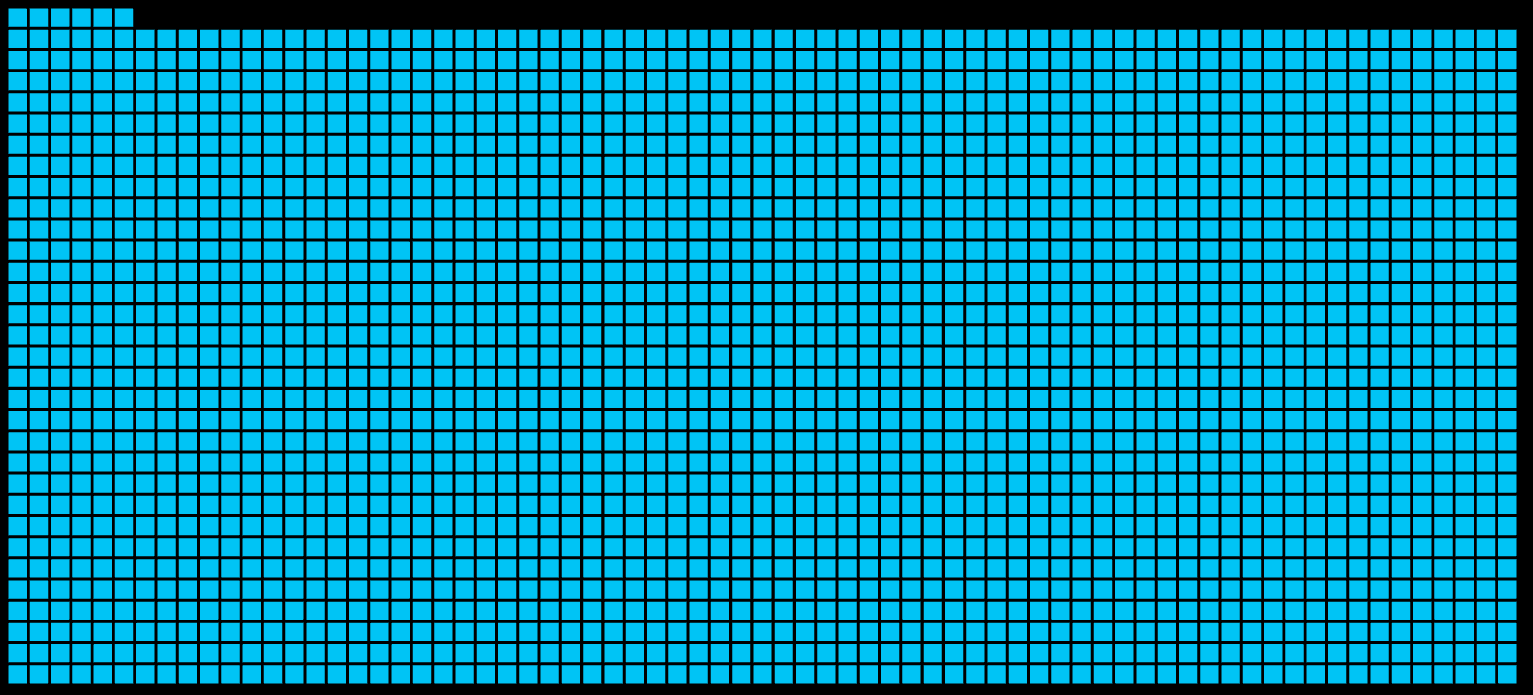
\includegraphics[height=5cm]{images/methods/related/sanddance-grid.png}
\caption[
    Unit-based grid in SandDance.
]{Unit-based grid in SandDance}
\label{fig:sanddance-grid}
\end{figure}

\ditem{Dot map} \hfill \\
Chapter \ref{s:dot} on page \pageref{s:dot} discusses the concept of dot maps in detail. This kind of thematic map can be used in combination with a one-to-one relationship and show every item in the dataset as a single dot on the map giving an overview of the whole dataset including its geographical distribution.

\ditem{Particle attractor} \hfill \\
Figure \ref{fig:particle-attractor} on page \pageref{fig:particle-attractor} sketches the concept of showing all data items around a particle attractor as an overview.

\begin{figure}[!htb]
\centering
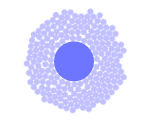
\includegraphics[height=5cm]{images/methods/related/particle-attractor.png}
\caption[
    Particle attractor sketch.
]{Particle attractor sketch}
\label{fig:particle-attractor}
\end{figure}

\end{enumerate}

The next step after having an overview is to decide which tasks to try out in order to test particle aggregation. One big part of this thesis already discusses thematic cartography in detail and thus the decision of using different types of thematic maps, which are all based on some kind of aggregation, is reasonable. Therefore trying animated particle aggregation in combination with proportional symbol maps, choropleth maps and cartograms will be a main part of the practical approach. However, there are multiple ways in changing visual appearance from an overview of the data to some kind of thematic map.

\begin{enumerate}

\ditem{In-place transition} \hfill \\
Changing from one kind of a thematic map to another one with in-place transition denotes the concept of creating the upcoming visualisation. Starting with an overview grid and having a dot map as an upcoming visualisation would move all particles in the same canvas to their geographical position. Having a map in the background when changing from an abstract grid to a thematic map could support the comprehensibility.
If the user determines to change the visual appearance to some other kind of thematic map, the particles would need to move according to the characteristics of the upcoming visualisation. Without consideration of using other visual channels except motion, in-place transitions have multiple advantages:
\begin{itemize}
\item Semantic constancy
\item Amount of particles stays the same throughout the application (this becomes more clear when reading non in-place transitions)
\end{itemize}

\ditem{Non in-place transitions} \hfill \\
Animating the transition from one thematic map to another can also be done with an adaption of the multiple views concept. \citeauthor{Javed2012} present different visualisation compositions which can be adopted for animated transitions as well \iacite{Javed2012}:
\begin{itemize}
\item \textbf{Juxtaposition:} placing visualisations side-by-side in one view
\item \textbf{Superimposition:} overlaying two visualisations in one view
\item \textbf{Overloading:} utilizing the space of one visualisation
\item \textbf{Nesting:} nesting the contents of one visualisation inside another one
\end{itemize}

All of the mentioned compositions can be accomplished in two different ways. Either each particle updates its position according to the upcoming visualisation, or each particle is cloned, and the clone updates its position accordingly. The latter method has the major drawback of scaling poorly because a dataset with $n$ items would need $2*n$ particles when changing the visual appearance.
\end{enumerate}

Both transition types perhaps share the same advantage: using some kind of animated transition between two different visual appearances for the same data could support the readability of the visualisation. Howsoever the particles move, it could help to understand how the visualisation is created and therefore could support knowledge construction.
However, starting with a particle attractor as an overview, it is also possible to use this attractor to animate the creation and transition of visualisations. Creating marks on a visual representation could be done in two ways:

\begin{enumerate}
\item Each particle tags its spot on the map by leaving an abstract, static mark
\item Each particle moves to its spot on the map and stays
\end{enumerate}

The first method would yield animated creations, with a very basic approach when changing the visual appearance. All particles would draw upcoming visualisations every time, without considering some kind of transition from the first to the second one. The second approach can be used to initially draw the first thematic map when no other visualisation is given. Changing the visual appearance if a thematic map is already shown, the mentioned transition methods can be used.

\begin{figure}[!htb]
\centering
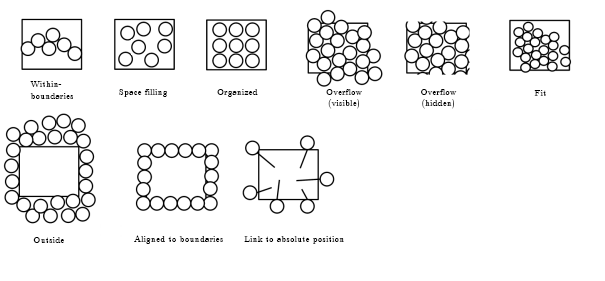
\includegraphics[height=5cm]{images/methods/related/strategies.png}
\caption[
    Particle design strategies to fit in or interact with a perimeter.
]{Particle design strategies to fit in or interact with a perimeter.}
\label{fig:particle-design-strategies}
\end{figure}

Considering the transition from a dot map to any other type of thematic map, the aggregation needs to be animated. Figure \ref{fig:particle-design-strategies} on page \pageref{fig:particle-design-strategies} shows nine different ways of how particles are able to fit in or interact with a perimeter of a given abstract shape. This heavily influences the movement of particles and the readability of the map. Aggregation can not only be done by moving the particle to their new aggregated shape. It could also be accomplished by using the concept of visual sedimentation, but it would also inherit its major weakness of not showing a static when using static data. When using the concept of SandDance of building aggregated shapes with units, a map will suffer from overplotting in high-density region, thus leading to visual clutter. Therefore most of the shown unit design strategies will be unusable in combination with certain thematic maps, e.g. proportional symbol maps.

Table \ref{tab:transition-table} on page \pageref{tab:transition-table} shows some concepts of animated transitions between visual appearances. Every concept is described with an abbreviation in the table which is explained in detail in the description list below. If the table mentions two methods in a cell, it means that there are two possible options available as an animated transition method.

\begin{table}[!htp]
    \begin{tabular}{M{22mm}||M{22mm} | M{22mm} | M{22mm} | M{22mm} | M{22mm} N}

    ~                       & Overview & Dot Map & Proportional Symbol Map & Choropleth Map & Cartogram &\\[4ex] \hline \hline

    Overview                & ~        & Linear       & Dot                       & Dot              & Dot         &\\[4ex] \hline

    Dot Map                 & Linear        & ~       & CB-Linear                       & Color-Linear              & CB-Linear         &\\[4ex] \hline

    Proportional Symbol Map & Dot        & CB-Linear       & ~                       & Dot, Shape              & Dot, Symbol         &\\[4ex] \hline

    Choropleth Map          & Dot        & Color-Linear       & Dot, Shape                       & ~              & Dot, Shape         &\\[4ex] \hline

    Cartogram               & Dot        & CB-Linear       & Dot, Symbol                       & Dot, Shape              & ~         &\\[4ex]
    \end{tabular}
    \caption{Transition table showing a transition from a given visualisation (column) to any upcoming visualisation (rows)}
    \label{tab:transition-table}
\end{table}

\begin{description}

\item[CB-Linear] \hfill \\
Centroid-based linear transition denotes that particles move to their geographical centroid and aggregate after moving. The aggregation can be accomplished with any kind of fitting or interacting with a perimeter.

\item[Color-Linear] \hfill \\
Color-linear transition can be implemented in two different ways:
\begin{enumerate}
\item Each particle leaves a blur of colour in its area. If more than one particle exists in a certain enumeration unit, the particles blur the area consecutively. Thus each particle increases the color intensity of the enumeration unit.
\item The particles simply fade out and the enumeration units get coloured.
\end{enumerate}

\item[Dot] \hfill \\
Dot-based transition means a simple linear transition to the dot map. The desired upcoming visualisation is then animated with the dot map as starting point. Therefore this transition implies two transitions. For example, \textit{Overview} to \textit{Proportional Symbol Map} is listed with a \textit{Dot}-transition in the table. This means that all particles are first animated with a linear transition to the dot map, followed by a centroid-based linear transition to the proportional symbol map. Thus, if the table denotes \textit{Dot} as an available transition method, the upcoming transition needs to be looked up in the dot map column in order to know the full transition.

\item[Linear] \hfill \\
This transition is characterized by an exact linear transition according to the spatial location.

\item[Shape] \hfill \\
Animating shape transition from e.g. a proportional symbol to an enumeration unit is abbreviated with "Shape" in the table.

\item[Symbol] \hfill \\
Animating the symbol is close related to animate the shape, except that the desired visualisation is not based upon enumeration units, therefore giving it a separate name seems appropriate.

\end{description}

At the beginning of this section, it is mentioned that the requirement of an interactive web application is given. However, this requirement needs to distinguish two different concepts of web applications:
\begin{enumerate}

\ditem{Pure client-side web application} \hfill \\
A client typically is a computer application, that runs on a user's local computer. With the context of a web application, a client is basically a web browser. In order to reach a web application, a client needs to connect to a server. With a pure client-side concept, the server returns static files only, thus leaving all further operations and calculations with the application on the client. The main advantage of such a concept is, that server costs can be significantly decreased and latency is basically not given when the first connection has been established. However, using the client for all further operations can be either an advantage or disadvantage, depending on the client's performance. If the client's hardware can handle a lot of operations, the web application will be extremely fast. However, if this is not the case and calculations, animations, etc. will take some time to be done, it will feel unnatural and unrewarding.

\ditem{Client-side web application combined with a server} \hfill \\
SandDance uses such a concept for its unit-based visualisation tool. The main difference to pure client-side web applications is, that operations and calculations are done on the server and the results are forwarded to the client. The client is only used to display information with animations and other concepts. This concept of a web-application needs a more abstract structure because client-server communication is obligatory. The information exchange will not affect a client in any way if the latency between a client and a server can be kept really low and the server has enough resources to perform fast.
\end{enumerate}
